\documentclass[main.tex]{subfiles} 
\begin{document}

\section{VIDEO COMPREHENSION SCORE (VCS): A METRIC FOR LONG-FORM VIDEO DESCRIPTION EVALUATION}

\begin{figure*}[t]
\centering
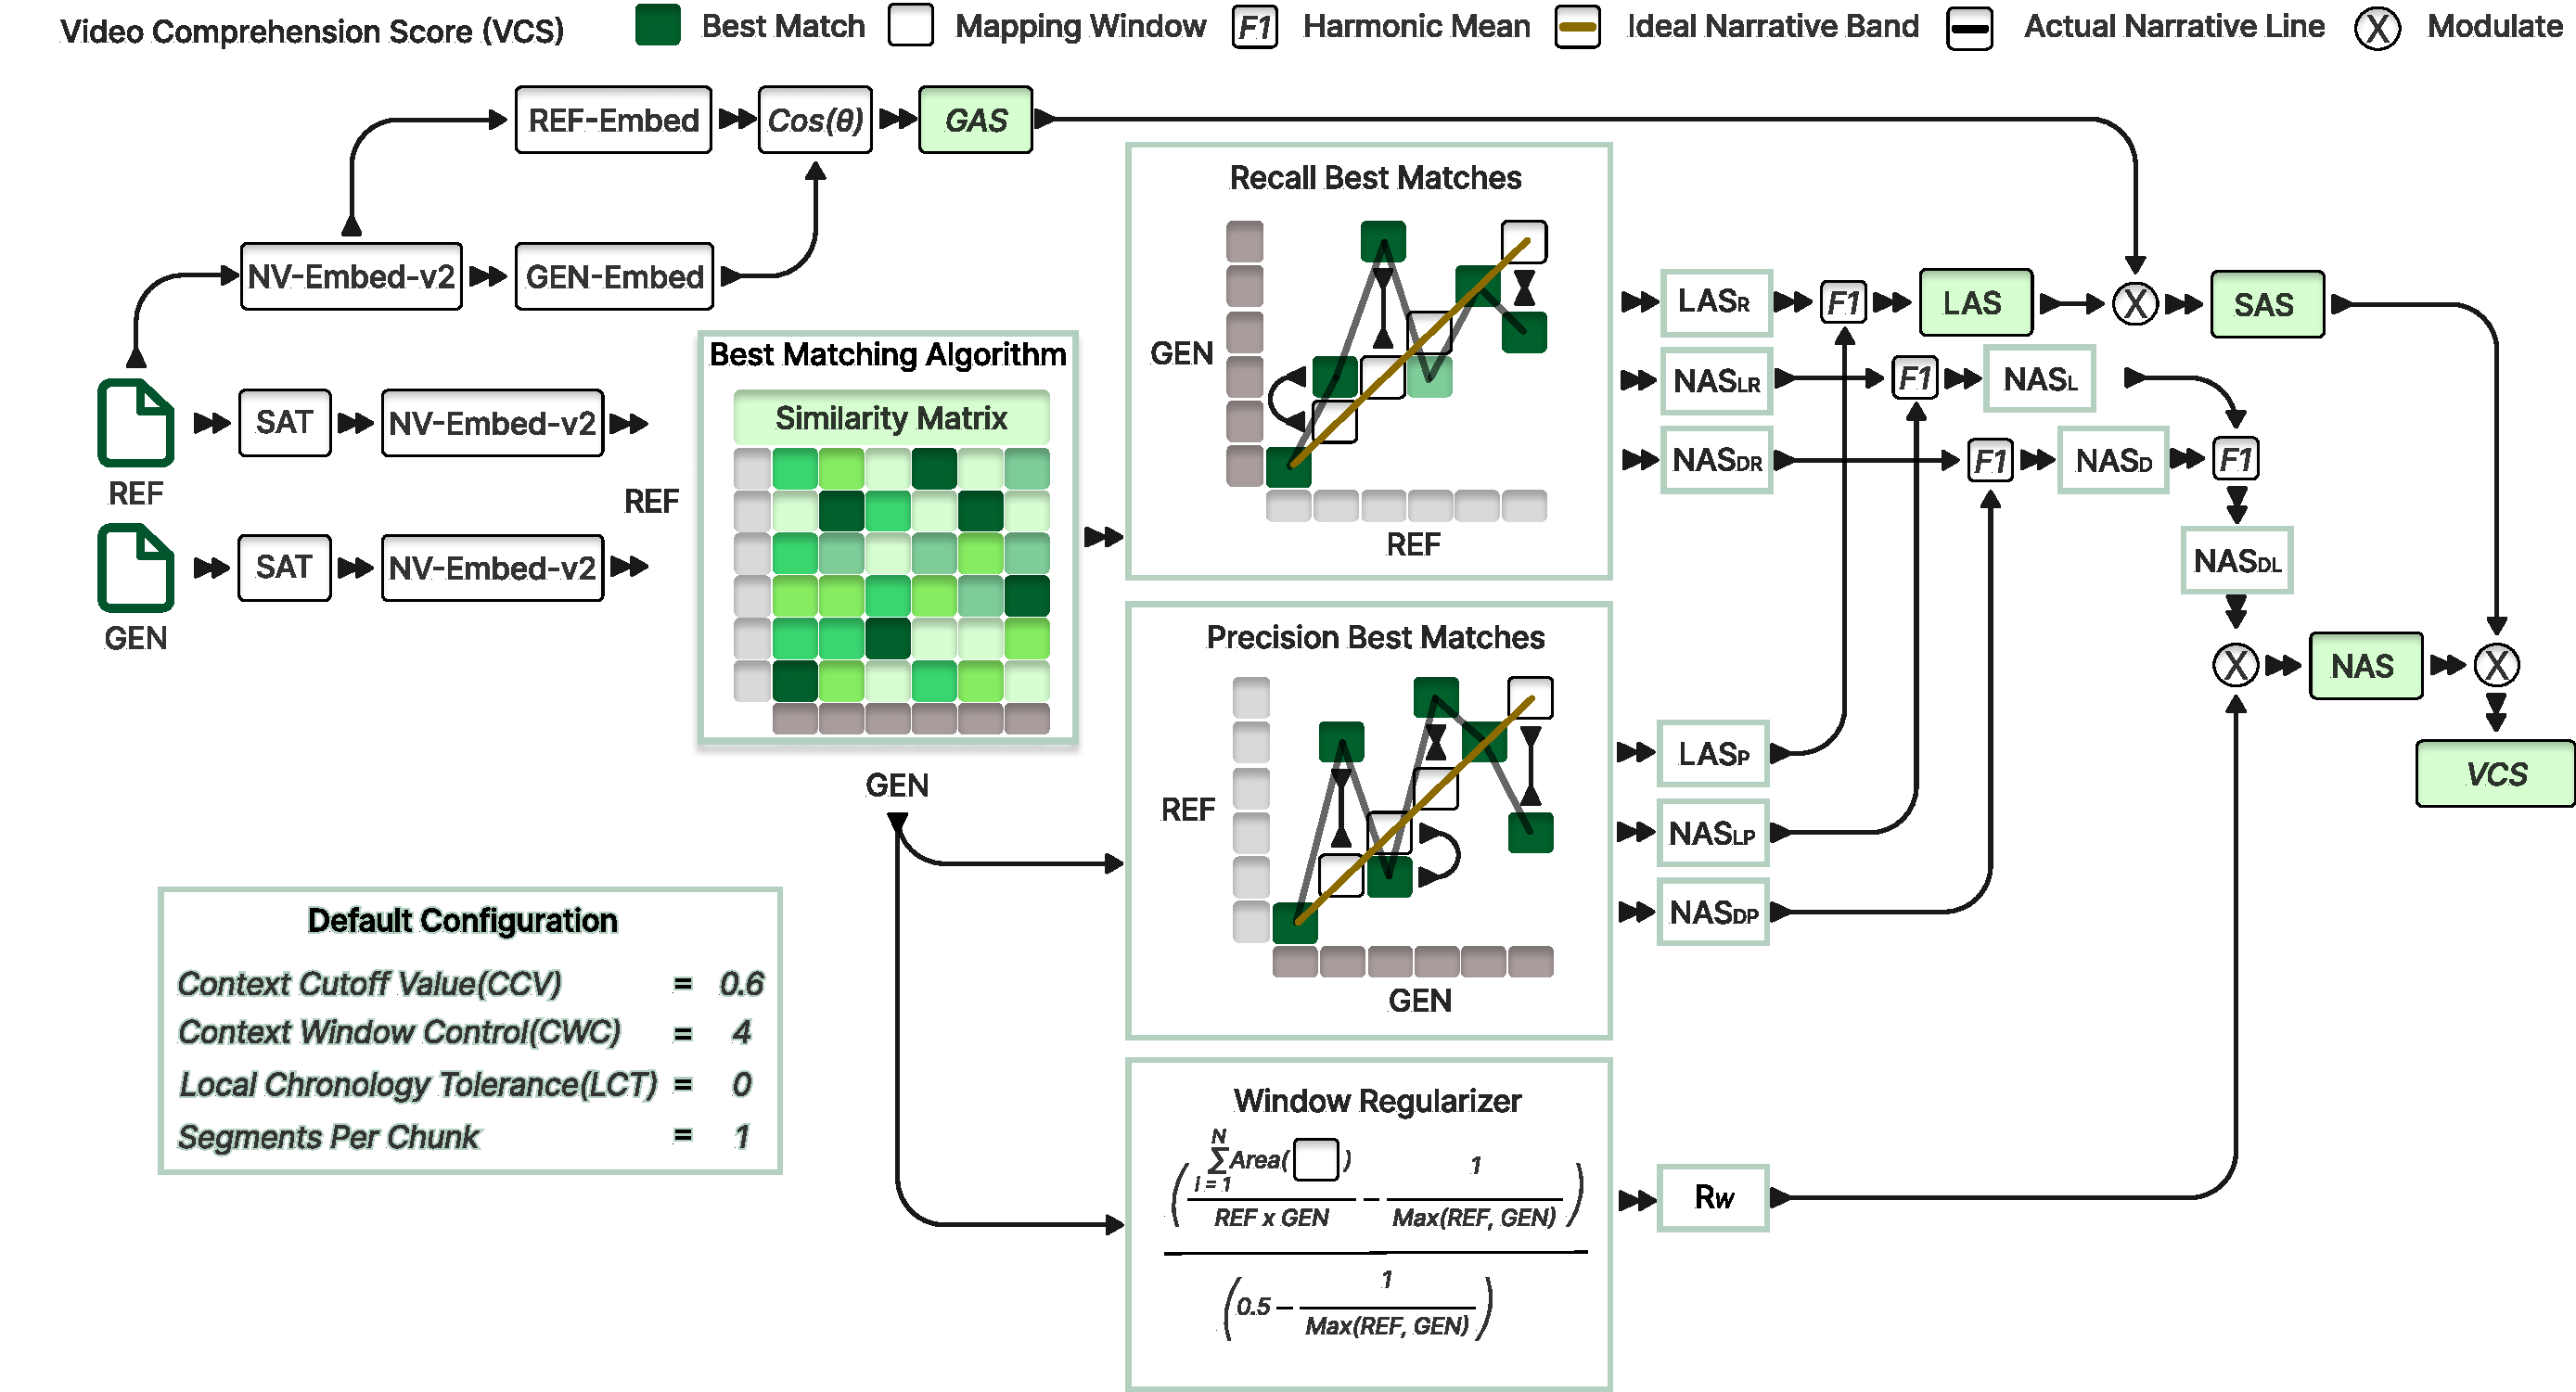
\includegraphics[width=0.8\textwidth]{images/VCS.pdf}
\caption{VCS Pipeline. The VCS assesses video descriptions by comparing a reference text ($T_{ref}$) with a model-generated text ($T_{gen}$). Both texts are initially segmented by SaT and embedded via NV-Embed-v2. The Global Alignment Score (GAS) is computed from the full text embeddings. For localized analysis, texts are chunked and embedded, forming a similarity matrix. From this, precision and recall-oriented best matches yield the Local Alignment Score (LAS)—the harmonic mean of $LAS_P$ (precision) and $LAS_R$ (recall). The Narrative Alignment Score (NAS) incorporates distance-based ($NAS_D$) and line-based ($NAS_L$) assessments. $NAS_D$ and $NAS_L$ are harmonic means of their respective precision and recall components. A Window Regularizer ($R_W$) refines the NAS. The Semantic Alignment Score (SAS) is derived by modulating GAS with LAS. The final VCS results from modulating the smaller of SAS and the regularized NAS with the larger.}
\label{fig:vcs-architecture}
\end{figure*}

\subsection{INTRODUCTION}

Recent advancements in Large Video Language Models (LVLMs) \cite{Yuan2025Tarsier2,Shen2025LongVU,Ataallah2024Goldfish,Chen2025LongVILA} have enhanced automated video comprehension, enabling long-form description generation from long videos. However, exploratory analysis on long videos reveals that LVLMs frequently (i) miss global narrative structure, (ii) fail to capture local events, and (iii) fail to establish temporal connections while hallucinating content. These gaps indicate LVLMs lack true video comprehension, raising the question: how can we evaluate models' video comprehension? Current benchmarks utilize question-answering formats \cite{wu2024longvideobench,ataallah2024infinibench,nagrani2025neptune} or short-form description comparisons for short videos \cite{wyzs:24,chen:acl11,ZhXuCoAAAI18}, both inadequate to evaluate models' true video comprehension ability. Evaluating genuine comprehension demands shifting to a methodology that processes long or complex videos and requires models to generate long-form descriptions. This approach renders superficial frame-level analysis insufficient, compelling models to instead generate outputs that capture global narrative structure, detail specific local events, and establish their temporal relationships. The quality of these generated descriptions can then be evaluated against the source video or human-written descriptions.

Description-based evaluation methods fall into four categories, each struggling with fundamental aspects of long-form evaluation. N-gram metrics such as BLEU \cite{p:02}, METEOR \cite{bl:05}, CIDEr \cite{v:15}, and ROUGE \cite{l:04} rely on lexical overlap, which not only unfairly penalizes legitimate paraphrases but also rewards superficial word-level matches between descriptions with entirely different global narratives. Embedding-based metrics like BERTScore \cite{z:20} and SBERT \cite{r:19} address lexical limitations through semantic similarity but overlook chronological alignment and local fine-grained details, allowing misordered events and subtle errors to remain undetected. Multimodal metrics such as EMScore \cite{syxl:22} enable direct comparison against source video content but struggle with long videos and long-form descriptions. LLM-based metrics such as CLAIR \cite{chan:23} and AutoDQ \cite{wyzs:24} provide deeper insights but often do not evaluate the chronology of events while suffering from consistency issues.

To address these limitations, we introduce VCS with three components:
\begin{enumerate}
\item \textbf{Global Alignment Score (GAS)}: Measures global thematic alignment.
\item \textbf{Local Alignment Score (LAS)}: Assesses local semantic alignment.
\item \textbf{Narrative Alignment Score (NAS)}: Evaluates chronological alignment using configurable Local Narrative Tolerance (LNT).
\end{enumerate}

VCS combines these three components to provide comprehensive evaluation: GAS and LAS form the Semantic Alignment Score (SAS), which integrates with NAS to produce the final VCS score. We also present VCS$_{\text{short}}$, which applies the same framework to short-form descriptions.

To evaluate VCS, we need datasets of long-form video descriptions paired with quality assessments—but no such datasets exist. Although creating a human-annotated dataset with quality ratings would be ideal, it is impractical: producing and reviewing long-form descriptions is costly and time-consuming, and annotator agreement declines sharply as description length increases. We therefore constructed a large-scale synthetic dataset from the MPII Movie Description Dataset \cite{rohrbach2015dataset} via ChatGPT-4o. From this dataset, we derived two test sets: a Corruption Detection Test Set to evaluate VCS ability to distinguish valid variations from invalid corruptions, and a Cross-Author Consistency Test Set to assess robustness across different authorial styles. VCS consistently outperforms traditional metrics on corruption detection tasks. To assess human correlation, we evaluate VCS$_{\text{short}}$ on VATEX-EVAL \cite{syxl:22}, where it achieves state-of-the-art results. These results demonstrate VCS effectiveness for robust evaluation of both long-form and short-form video descriptions.

Our primary contributions include:
\begin{itemize}
\item A robust metric (VCS) for both long-form and short-form video descriptions.
\item Configurable LNT and chunk size parameters to govern chronological strictness and comparison granularity.
\end{itemize}

\subsection{RELATED WORK}

Traditional n-gram-based metrics such as BLEU \cite{p:02}, ROUGE \cite{l:04}, and METEOR \cite{bl:05} evaluate text generation through lexical overlap and local word order. BLEU measures n-gram precision with brevity penalties, capturing local ordering but missing event-level chronology and struggling with expressive variability. ROUGE variants compute precision, recall, and F1-scores: ROUGE-N evaluates n-gram overlap, ROUGE-L computes Longest Common Subsequence at summary-level, and ROUGE-Lsum calculates sentence-level LCS by splitting at newlines. While preserving sequential information, they miss event-level chronology and remain sensitive to expressive variability. METEOR addresses expressive variability via synonyms and stems, computing recall-weighted F-scores with fragmentation penalties, but similarly misses event-level chronology. CIDEr \cite{v:15} uses consensus-based TF-IDF weighting across multiple references but proves impractical for long-form descriptions due to labor-intensive annotation. SPICE \cite{afjg:16} evaluates semantic propositions using graph overlaps, effectively handling paraphrasing; however, being designed for static images, it cannot be directly applied to videos and neglects narrative chronology critical for video descriptions.

Embedding-based metrics compare texts in semantic vector spaces, leveraging pretrained models to capture semantic similarity beyond lexical matches. BERTScore computes token-level similarity using contextualized BERT embeddings, aggregating optimal alignments into precision, recall, and F1-scores, while SBERT employs siamese networks with mean-pooling for sentence-level embeddings, but both address expressive variability by recognizing paraphrases yet are constrained by limited context windows, complicating their direct application to long-form descriptions. Recent decoder-based models such as NV-Embed-v2 \cite{l:24}, Linq-Embed-Mistral, SFR-Embedding-Mistral, and Jasper and Stella leverage autoregressive LLM architectures with bidirectional attention, offering significantly larger context windows and robust global embeddings, excelling at paragraph-level semantic assessments. However, reliance on global embeddings and cosine similarity overlooks local content alignment, detailed information accuracy, and chronological alignment.

Multimodal embedding metrics like EMScore \cite{syxl:22} and PAC-S employ vision-language models such as CLIP \cite{Radford2021LearningTV} to evaluate semantic alignment between visuals and generated captions, addressing expressive variability through direct image-caption comparison, thus bypassing reference captions. EMScore computes video-caption similarity through dual-level matching: coarse-grained alignment between video and caption embeddings, and fine-grained matching between frames and words, calculating precision, recall, and F1-scores via cosine similarity. PAC-S fine-tunes CLIP through positive-augmented contrastive learning with synthetic image-text pairs, then computes cosine similarity scores from the enhanced model. Despite their effectiveness in short-form descriptions, these metrics face computational challenges and methodological limitations when scaling to long-form descriptions.

Recent evaluation approaches increasingly leverage Large Language Models (LLMs), categorized into component-based and holistic judge methods. Component-based methods such as AutoDQ \cite{wyzs:24} extract events from descriptions using ChatGPT, then compute precision and recall through entailment analysis comparing extracted events between texts, while VAD-Score employs LLMs for semantic extraction and scoring of events, subjects, and objects, effectively addressing expressive variability but missing chronological evaluation. Holistic methods such as CapScore prompt GPT-4 to score caption similarity and quality, CapArena-Auto Score uses GPT-4o for pairwise evaluation battles, and CLAIR \cite{chan:23} employs zero-shot prompting for similarity scores with interpretable reasoning. However, these methods suffer from ambiguity in score calibration, sensitivity to prompting nuances, consistency issues across model versions, limited interpretability, and practical constraints including reproducibility and cost.

\subsection{METHODOLOGY}
\label{sec:methodology_vcs}

Figure~\ref{fig:vcs-architecture} shows the VCS pipeline, which computes semantic and narrative alignment between reference and generated descriptions to achieve comprehensive long-form video description evaluation.

\subsubsection{Global Alignment Score (GAS)}
VCS computes GAS to capture global thematic alignment between reference and generated descriptions. Given input texts $T_{ref}$ and $T_{gen}$, we encode each description using NV-Embed-v2. The GAS is computed as:

\begin{equation} \label{eq:gas_revised}
\text{GAS} = \frac{\mathbf{E}_{ref} \cdot \mathbf{E}_{gen}}{\|\mathbf{E}_{ref}\| \|\mathbf{E}_{gen}\|}
\end{equation}

\subsubsection{Text Preprocessing for Chunk-Level Analysis}
However, GAS lacks sensitivity to fine-grained details and chronological consistency. To enable fine-grained analysis, VCS applies punctuation removal and Segment Any Text (SaT)~\cite{frohmann-etal-2024-segment} segmentation to $T_{ref}$ and $T_{gen}$, producing semantic segments $S_{ref}$ and $S_{gen}$. We group $k$ consecutive segments into chunks $C_{ref} = \{c_1^{ref}, ..., c_{N_{ref}}^{ref}\}$ and $C_{gen} = \{c_1^{gen}, ..., c_{N_{gen}}^{gen}\}$, embedded using NV-Embed-v2 to yield matrices $\mathbf{E}_{C_{ref}} \in \mathbb{R}^{N_{ref} \times D}$ and $\mathbf{E}_{C_{gen}} \in \mathbb{R}^{N_{gen} \times D}$.

\subsubsection{Defining Mapping Windows}
Before establishing chunk correspondences for fine-grained assessment, VCS constructs a similarity matrix to enable optimal alignments. Using $\mathbf{E}_{C_{ref}}$ and $\mathbf{E}_{C_{gen}}$, we compute similarity matrix $\mathbf{S} \in \mathbb{R}^{N_{ref} \times N_{gen}}$ where $S_{i,j} = \cos(\mathbf{E}_{C_{ref}}[i], \mathbf{E}_{C_{gen}}[j])$ represents the cosine similarity between the $i$-th reference chunk and $j$-th generated chunk.

However, before selecting the best match for each chunk, VCS defines Mapping Windows (MW) that constrain the search space within this similarity matrix. This concept stems from empirical observations: when computing pairwise chunk embeddings between identical long-form descriptions, the resulting similarity matrix exhibits a clear diagonal structure where $C_1^{ref}$ maps to $C_1^{gen}$, $C_2^{ref}$ maps to $C_2^{gen}$, and so on, with this diagonal pattern stretching or compressing proportionally in brevity or verbosity cases. Hence, for given chunk counts $N_{ref}$ and $N_{gen}$, we define this diagonal search space and call it Mapping Windows—regions where each chunk should ideally map.

VCS identifies the longer sequence as $\max(N_{ref}, N_{gen})$ and the shorter sequence as $\min(N_{ref}, N_{gen})$. We compute slope $s = \text{longer}/\text{shorter}$ and base window height $h_{mw} = \lceil s \rceil$. The algorithm creates direct windows by mapping each position $i$ in the shorter sequence to a window of height $h_{mw}$ in the longer sequence, spanning range $[\lfloor i \cdot s \rfloor, \min(\lfloor i \cdot s \rfloor + h_{mw}, \text{longer}))$ with proportional scaling. Reverse windows invert this mapping: for each position in the longer sequence, we determine which positions in the shorter sequence include it. VCS assigns Precision Windows ($MW_p$) and Recall Windows ($MW_r$) based on sequence direction: when $N_{ref} \geq N_{gen}$, precision uses direct windows and recall uses reverse windows; otherwise, assignments are reversed.

\subsubsection{Best Matching Algorithm}
Having established Mapping Windows within the similarity matrix $\mathbf{S}$, VCS pairs each generated chunk with its best reference counterpart, and vice versa. Naively selecting the highest-similarity reference for each generated chunk leads to semantic collision and semantic ambiguity. Semantic collision occurs when a single chunk exhibits identical similarity to multiple counterparts, while semantic ambiguity arises when a chunk achieves nearly equal similarity with multiple candidates. Both issues stem from repeated events or superficial lexical overlap, obscuring true narrative counterparts.

VCS resolves these issues through a Best-Matching Algorithm that combines adaptive context filtering with mapping-window constraints. Adaptive context filtering first determines a candidate set around the maximum similarity rather than committing immediately to the top score. Two user-defined parameters control this process: the context cutoff $\tau_{ctx}$ (default 0.6) and the context window control $k_{ctx}$ (default 4). Similarities below the cutoff receive no context expansion, while those above it define a context window whose width is computed as

\begin{equation}
w_{ctx} = \frac{(1-\tau_{ctx})-(1-s_{max})}{s_{max} \cdot k_{ctx}},
\end{equation}

where $s_{max}$ is the maximum similarity for the chunk. All candidates within $s_{max} - w_{ctx}$ enter the pool for selection. Mapping-window constraints then enforce temporal alignment: among the candidate matches, the algorithm chooses the chunk closest to the mapping-window boundary of the target chunk, breaking ties by similarity. When $s_{max}$ falls below the cutoff, no context expansion occurs, and ties are resolved purely by distance from the mapping-window boundary.

This combination mitigates both collision and ambiguity. Executing this procedure for each generated chunk and each reference chunk yields precision best matches $M_P = \{(C_j^{gen}, C_{i^*}^{ref})\}$ and recall best matches $M_R = \{(C_i^{ref}, C_{j^*}^{gen})\}$.

\subsubsection{Local Alignment Score (LAS)}
Having obtained the correspondence sets $M_P$ and $M_R$ from the Best-Matching Algorithm, VCS computes the LAS by averaging cosine similarities of matched chunk pairs. The precision component $LAS_P$ evaluates how well generated text aligns with reference text, while recall component $LAS_R$ evaluates the reverse. LAS is their harmonic mean:

\begin{equation}
LAS = \frac{2 \cdot LAS_P \cdot LAS_R}{LAS_P + LAS_R}
\end{equation}

\subsubsection{Narrative Alignment Score (NAS)}
However, LAS remains insensitive to chronological ordering and exhibits limited sensitivity to missing or extra content. While LAS performs local semantic alignment and can detect content variations, its reliance on semantic similarity averaging means that even weak semantic matches contribute to the overall score, reducing its ability to strongly penalize missing or extraneous content. To mitigate both limitations, VCS introduces NAS that evaluates chronological consistency while enhancing sensitivity to content gaps and additions through narrative alignment assessment. NAS comprises four components: Distance-based NAS ($NAS_D$), Line-based NAS ($NAS_L$), a window regularizer, and the user-controlled Local Narrative Tolerance (LNT) parameter.

\subsubsection{Defining Local Narrative Tolerance (LNT)}
Before assessing narrative alignment, VCS defines a user-controlled parameter called LNT. This concept stems from the observation that video narratives often permit multiple valid orderings and descriptive variations where temporally adjacent or concurrent events can be described in different sequences and detail levels without compromising narrative coherence. Complex video scenes frequently contain multiple actors and objects performing concurrent actions, where these details can be expressed in multiple valid orders and varying descriptive granularity—from highly detailed to moderate to sparse descriptions. To accommodate this inherent flexibility, VCS employs LNT as a tolerance parameter that defines acceptable deviation from strict chronological order and descriptive consistency, allowing higher LNT values to provide tolerance for both narrative reordering and descriptive variability when dense descriptions describe scenes with slightly different detail levels.

\subsubsection{Distance-based NAS ($NAS_D$)}
Mapping Windows define where chunks should ideally match if the narrative structure is preserved between reference and generated descriptions. $NAS_D$ formalizes this intuition by penalizing each chunk based on its distance from the ideal region defined by the Mapping Windows. For precision evaluation, $NAS_D$ uses correspondence set $M_P$ and precision Mapping Windows $MW_p$; for recall evaluation, it uses correspondence set $M_R$ and recall Mapping Windows $MW_r$.

However, before computing penalties, VCS applies Local Narrative Tolerance (LNT) to account for natural narrative variations. LNT expands each Mapping Window with penalty-free zones, recognizing that chunks matching within these expanded regions represent acceptable chronological alignments. We first compute the LNT window height:

\begin{equation}
h_{LNT} = \lceil y/x \rceil - 1[y > x \land 0 < \text{frac}(y/x) \leq 0.5]
\end{equation}

where $y = N_{ref}$ and $x = N_{gen}$ for $NAS_{D,prec}$, and the reverse for $NAS_{D,rec}$. A user-defined multiplier $\tau_{LNT} \geq 0$ expands each Mapping Window by $\tau_{LNT} \cdot h_{LNT}$ rows. Chunks matching within this expanded window receive zero penalty.

For chunks outside this tolerance zone, distance penalties are calculated from their offset from the Mapping Window boundary. Each evaluation chunk has a corresponding Mapping Window; if the matched chunk appears above the window, the raw offset measures rows above the window start; if below, it measures rows below the window end. The penalty becomes zero if this offset falls within the LNT tolerance, otherwise it equals the offset normalized by timeline length.

Let $P_{total}$ sum all penalties across matched pairs and $P_{max}$ represent the worst-case penalty when all chunks drift to furthest positions. The orientation score is computed as:

\begin{equation}
NAS_{D,*} = 1 - \frac{P_{total}}{P_{max}}
\end{equation}

For precision, $eval = gen$, $opp = ref$, $M_{eval} = M_P$, and $MW_{eval} = MW_p$; for recall, $eval = ref$, $opp = gen$, $M_{eval} = M_R$, and $MW_{eval} = MW_r$. The final score combines both orientations:

\begin{equation}
NAS_D = \frac{2 \cdot NAS_{D,prec} \cdot NAS_{D,rec}}{NAS_{D,prec} + NAS_{D,rec}}
\end{equation}

\subsubsection{Line-based NAS ($NAS_L$)}
Treating each matched pair as a vertex $(x_i, y_i)$, VCS compares the path that connects them to an ideal narrative band bounded by the shortest and longest feasible paths constrained by the Mapping Windows. Dynamic programming gives the floor length $L_{min}$ and ceil length $L_{max}$; their vertical increments $\Delta y_{x_i}^{\text{floor}}$ are cached for later clipping. With source length $N_{src}$ and target length $N_{tgt}$ (equal to $N_{ref}$ or $N_{gen}$ depending on orientation) the base window height is $h_{mw} = \lceil N_{tgt}/N_{src} \rceil$. This height in turn defines an LNT kernel $\omega_0$ and its expanded version $\omega_{LNT} = \omega_0 + \kappa \tau_{LNT}$, where the scale $\kappa$ is $h_{mw}$ or $h_{mw} - 1$ exactly as in the implementation. For consecutive vertices the segment length is

\begin{equation}
\ell_i = \begin{cases}
\sqrt{\Delta x_i^2 + \Delta y_i^2}, & 0 \leq |\Delta y_i|^* \leq \omega_0, \\
\sqrt{\Delta x_i^2 + |\Delta y_{x_i}^{\text{floor}}|^2}, & \omega_0 < |\Delta y_i|^* \leq \omega_{LNT}, \\
0, & \text{otherwise},
\end{cases}
\end{equation}

where $|\Delta y_i|^* = |\Delta y_i|$ if $\tau_{LNT} > 0$ and $|\Delta y_i|^* = \Delta y_i$ when $\tau_{LNT} = 0$. Summing $\ell_i$ gives the realised length $L_{act}$. The orientation score is

\begin{equation}
NAS_{L,*} = \begin{cases}
1, & L_{min} \leq L_{act} \leq L_{max}, \\
L_{act}/L_{min}, & L_{act} < L_{min}, \\
L_{max}/L_{act}, & L_{act} > L_{max}.
\end{cases}
\end{equation}

The two orientations are again combined with a harmonic mean to obtain $NAS_L$.

\subsubsection{Window-area Regulariser ($R_w$)}
Let $W$ be the Mapping-Window set that spans the longer vertical timeline ($MW_{rec}$ if $N_{gen} > N_{ref}$, otherwise $MW_{prec}$). With window heights $h_j$, the covered area is $A_{MW} = \sum_{w_j \in W} h_j$; the full grid area is $A_{timeline} = N_{ref} N_{gen}$. Setting $a = A_{MW}/A_{timeline}$ and $a_{min} = 1/\max(N_{ref}, N_{gen})$, we regularise the window width by

\begin{equation}
R_w = \text{clip}[(a - a_{min})/(0.5 - a_{min}), 0, 1].
\end{equation}

\subsubsection{Final NAS}
The distance- and line-based views are first merged: $NAS_{F1} = 2 NAS_D NAS_L/(NAS_D + NAS_L)$ (defined as 0 when both inputs are zero). Overly permissive windows are then discounted:

\begin{equation}
NAS_{final} = \begin{cases}
(NAS_{F1} - R_w)/(1 - R_w), & NAS_{F1} > R_w, \\
0, & \text{otherwise}.
\end{cases}
\end{equation}

Thus NAS captures positional fidelity ($NAS_D$), global path coherence ($NAS_L$), and penalises inflated scores that could arise from excessively wide Mapping Windows.

\subsubsection{Final VCS Aggregation}
The complete VCS integrates semantic and narrative alignment through careful score combination. GAS is modulated by LAS to yield Semantic Alignment Score ($SAS$):

\begin{equation} \label{eq:sas_revised} 
SAS = \frac{GAS - (1 - LAS)}{LAS}
\end{equation}

when $LAS > 0$ and the numerator is positive, otherwise $SAS = 0$. This ensures high global similarity requires supporting local semantic agreement. The final VCS uses adaptive weighting with intermediate variables:
\begin{align}
S_{min} &= \min(SAS, NAS_{final}) \label{eq:s_min} \\
S_{max} &= \max(SAS, NAS_{final}) \label{eq:s_max} \\
VCS &= \frac{S_{min} - (1 - S_{max})}{S_{max}} \label{eq:vcs_final}
\end{align}

when both components are positive and the numerator exceeds zero, otherwise $VCS = 0$.

\subsubsection{Extension for Short-Form Descriptions (VCS$_{short}$)}
For short-form description evaluation, VCS$_{short}$ adapts the complete VCS methodology to operate at word-level granularity. Input texts undergo cleaning to remove punctuation and stop words, then tokenization into individual words that serve as fundamental elements. These words replace multi-word chunks in all alignment and scoring processes while maintaining identical metric computation and aggregation logic, enabling consistent evaluation across different description lengths.

\subsection{DATASET CONSTRUCTION}

We construct two synthetic datasets from MPII-MD containing 94 movies with 68,000 annotated segments. We extract 1,390 consecutive scene groups (~500 words each) and use ChatGPT-4o to synthesize coherent narrative descriptions, yielding our base dataset.

\subsubsection{Corruption Detection Test Set}
We generate 10 valid variations and 10 invalid corruptions per base description to evaluate VCS ability to distinguish legitimate stylistic changes from content errors. Valid variations include lexical variation, voice transformation, paraphrasing, abstraction (50\%/70\% reduction), elaboration (130\%/150\% expansion), action decomposition/aggregation, and attribute injection while preserving narrative integrity. Invalid corruptions introduce content errors through SAO distortion, ID summarization, hallucination (50\%/80\% unrelated segments), omission (50\%/80\% deletion), sequence inversion, local/global permutation, and sequence rotation. All transformations employ SAT segmentation while preserving segment content integrity, producing 27,800 test instances.

\subsubsection{Cross-Author Consistency Test Set}
We use the same 1,390 scene groups with ChatGPT-4o as Author 1 baseline and prompt Grok 3, Claude Sonnet 3.5, and Mistral-Large to generate authorial variations. Each model applies systematic transformations including paraphrasing, voice switching, brevity/verbosity adjustments, action scaling, attribute modification, detail variation, and scene expansion while preserving chronological order and factual content. This produces 5,560 descriptions (1,390 × 4 authors) for evaluating metric robustness across writing styles.

\subsection{EXPERIMENTAL RESULTS}

We conduct comprehensive experiments to evaluate VCS performance on corruption detection tasks. Our evaluation compares VCS against established video description metrics to assess its ability to distinguish valid narrative variations from invalid corruptions.

We evaluate VCS alongside four rule-based metrics: BLEU, ROUGE-L, METEOR, and CIDEr, and two embedding-based metrics: BERTScore and SBERT. For BERTScore, we use the RoBERTa-base backbone with F1-measure configuration. For SBERT, we employ the all-MiniLM-L6-v2 model for sentence embeddings. VCS uses NV-Embed-v2 for text embeddings with chunk size $k=3$ and Local Narrative Tolerance $\tau_{LNT}=0.1$ across all experiments.

VCS consistently outperforms traditional metrics on corruption detection tasks, being the only metric capable of distinguishing valid variations from invalid corruptions. On cross-author consistency tasks, VCS is the only metric that consistently produces scores $>$80\% regardless of which authorial reference is used for evaluation. VCS$_{\text{short}}$ attains state-of-the-art human correlation on VATEX-EVAL in the 9-ref setting (Kendall's $\tau = 41.5$, Spearman's $\rho = 52.8$) and competitive results in the 1-ref setting (Kendall's $\tau = 30.0$, Spearman's $\rho = 38.1$). These results demonstrate VCS effectiveness for evaluating both long-form and short-form video descriptions.

\subsection{CONCLUSION}

We introduced VCS, a comprehensive evaluation metric for long-form video descriptions that addresses fundamental limitations of existing approaches. Through three core components—Global Alignment Score, Local Alignment Score, and Narrative Alignment Score—VCS provides robust evaluation of semantic alignment and chronological consistency. Our extensive experiments on synthetic datasets demonstrate VCS superior performance in corruption detection and cross-author consistency tasks, while VCS$_{\text{short}}$ achieves state-of-the-art human correlation results. This work establishes a foundation for reliable evaluation of video comprehension models and opens avenues for future research in automated video understanding assessment.

\end{document}